% ================================================================
%  FuzzyShield — Beamer Presentation  v2
%  Author: Ahmet Faruk Kesgin — 300201024
%  Compile: pdflatex presentation.tex  (run twice)
% ================================================================
\documentclass[aspectratio=169,12pt]{beamer}

% ── Packages ────────────────────────────────────────────────────────────────
\usepackage[T1]{fontenc}
\usepackage[utf8]{inputenc}
\usepackage[english]{babel}
\usepackage{lmodern}
\usepackage{graphicx}
\usepackage{booktabs}
\usepackage{array}
\usepackage{amsmath,amssymb}
\usepackage{xcolor}
\usepackage{tikz}
\usepackage{pgfplots}
\pgfplotsset{compat=1.17}
\usepackage{tabularx}
\usepackage{multirow}
\usepackage{caption}
\usepackage{hyperref}

% ── Colour Palette ──────────────────────────────────────────────────────────
\definecolor{iyte-blue}{RGB}{200,40,55}
\definecolor{iyte-light}{RGB}{252,230,230}
\definecolor{iyte-dark}{RGB}{160,25,38}
\definecolor{accent-r}{RGB}{220,50,50}
\definecolor{accent-t}{RGB}{150,105,0}
\definecolor{accent-c}{RGB}{148,103,220}
\definecolor{accent-g}{RGB}{40,160,80}
\definecolor{accent-m}{RGB}{0,125,170}

% ── Beamer Theme ─────────────────────────────────────────────────────────────
\usetheme{Madrid}
\usecolortheme[named=iyte-blue]{structure}

\setbeamercolor{palette primary}{bg=iyte-blue, fg=white}
\setbeamercolor{palette secondary}{bg=iyte-dark, fg=white}
\setbeamercolor{palette tertiary}{bg=iyte-blue!80, fg=white}
\setbeamercolor{palette quaternary}{bg=iyte-dark, fg=white}
\setbeamercolor{title}{fg=white}
\setbeamercolor{frametitle}{bg=iyte-blue, fg=white}
\setbeamercolor{block title}{bg=iyte-blue, fg=white}
\setbeamercolor{block body}{bg=iyte-light}
\setbeamercolor{block title alerted}{bg=accent-r, fg=white}
\setbeamercolor{block body alerted}{bg=accent-r!10}
\setbeamercolor{block title example}{bg=accent-g!80!black, fg=white}
\setbeamercolor{block body example}{bg=accent-g!10}
\setbeamercolor{itemize item}{fg=iyte-blue}
\setbeamercolor{itemize subitem}{fg=iyte-blue!70}
\setbeamercolor{section in toc}{fg=iyte-dark}
\setbeamercolor{subsection in toc}{fg=iyte-blue}

\setbeamerfont{title}{size=\Large, series=\bfseries}
\setbeamerfont{frametitle}{size=\large, series=\bfseries}
\setbeamerfont{block title}{size=\normalsize, series=\bfseries}

\setbeamertemplate{navigation symbols}{}
\setbeamertemplate{itemize item}{\textbullet}
\setbeamertemplate{itemize subitem}{--}

\setbeamertemplate{footline}{%
  \leavevmode%
  \hbox{%
    \begin{beamercolorbox}[wd=.33\paperwidth,ht=2.6ex,dp=1.2ex,left,leftskip=1em]{palette primary}%
      \usebeamerfont{author in head/foot}\insertshortauthor
    \end{beamercolorbox}%
    \begin{beamercolorbox}[wd=.34\paperwidth,ht=2.6ex,dp=1.2ex,center]{palette secondary}%
      \usebeamerfont{title in head/foot}\insertshorttitle
    \end{beamercolorbox}%
    \begin{beamercolorbox}[wd=.33\paperwidth,ht=2.6ex,dp=1.2ex,right,rightskip=1em]{palette primary}%
      \usebeamerfont{date in head/foot}%
      \insertframenumber{} / \inserttotalframenumber
    \end{beamercolorbox}%
  }%
}

% ── Helpers ─────────────────────────────────────────────────────────────────
\newcommand{\R}[1]{\textcolor{accent-r}{\textbf{#1}}}
\newcommand{\T}[1]{\textcolor{accent-t}{\textbf{#1}}}
\newcommand{\C}[1]{\textcolor{accent-c}{\textbf{#1}}}
\newcommand{\G}[1]{\textcolor{accent-g}{\textbf{#1}}}
\newcommand{\M}[1]{\textcolor{accent-m}{\textbf{#1}}}

% ── Metadata ────────────────────────────────────────────────────────────────
\title[FuzzyShield]{%
  \textbf{FuzzyShield}\\[0.2em]
  \normalsize Real-Time Behavioral Malware Classification\\
  Using Fuzzy Logic}
\subtitle{Term Project Presentation}
\author[A.\ F.\ Kesgin]{%
  Ahmet Faruk Kesgin\\
  \small\mbox{300201024}}
\institute[IYTE]{%
  Department of Computer Engineering\\
  Izmir Institute of Technology}
\date{June 2026}
\titlegraphic{
\includegraphics[height=1.1cm]{figures/iyte_logo.png}}

% ════════════════════════════════════════════════════════════════════════════
\begin{document}

% ── TITLE ────────────────────────────────────────────────────────────────────
\begin{frame}[plain]
  \titlepage
\end{frame}

% ── OUTLINE ──────────────────────────────────────────────────────────────────
\begin{frame}{Outline}
  \tableofcontents
\end{frame}

% ════════════════════════════════════════════════════════════════════════════
\section{Introduction}

\begin{frame}{The Problem: Signatures Are Not Enough}
  \begin{columns}[T]
    \begin{column}{0.50\textwidth}
      \begin{alertblock}{Signature-Based Detection}
        \begin{itemize}\small
          \item Matches binary hashes / byte patterns
          \item Requires a \textbf{known sample} to exist first
          \item Fails on \alert{zero-day} \& polymorphic malware
          \item Recompiling the binary evades detection
        \end{itemize}
      \end{alertblock}
      \vspace{0.4em}
      \begin{block}{Zero-Day Reality}
        \small
        Average exploit-to-patch window: \textbf{70 days}.\\
        Signature databases are \textbf{useless} during this window.
      \end{block}
    \end{column}
    \begin{column}{0.46\textwidth}
      \begin{exampleblock}{Behavioral Analysis}
        \begin{itemize}\small
          \item Observes \emph{what a process does}
          \item CPU, disk I/O, network, entropy
          \item Works on \alert{unknown} samples
          \item Complements signatures
        \end{itemize}
      \end{exampleblock}
      \vspace{0.4em}
      \begin{block}{Key Insight}
        \small
        \R{Ransomware} always \textbf{encrypts files}.\\
        \T{Trojans} always \textbf{exfiltrate data}.\\
        \C{Miners} always \textbf{max out CPU}.\\[0.2em]
        \textit{Behaviour is hard to hide.}
      \end{block}
    \end{column}
  \end{columns}
\end{frame}

\begin{frame}{Why Fuzzy Logic?}
  \begin{columns}[T]
    \begin{column}{0.54\textwidth}
      \textbf{Behavioral metrics are inherently imprecise:}
      \begin{itemize}\small
        \item CPU = 78\% \;—\; normal \emph{or} malicious?
        \item fwrite = 85 MB/s \;—\; high \emph{or} extreme?
        \item Hard thresholds produce false positives
      \end{itemize}
      \vspace{0.5em}
      \textbf{Fuzzy sets handle the grey zones:}
      \begin{itemize}\small
        \item 78\% CPU $\;\Rightarrow\;$
              \texttt{high}(0.60), \texttt{extreme}(0.20)
        \item Smooth transitions, not hard cuts
        \item Human-readable IF-THEN rules
        \item \textbf{Transparent} — analyst can inspect every rule
      \end{itemize}
    \end{column}
    \begin{column}{0.42\textwidth}
      \begin{block}{Mamdani FIS Pipeline}
        \centering\vspace{0.3em}
        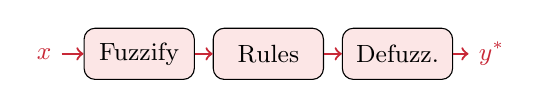
\begin{tikzpicture}[scale=0.82, font=\small,
            box/.style={draw, rounded corners, fill=iyte-light,
                        minimum width=1.4cm, minimum height=0.65cm}]
          \node[box] (fuzz)  at (0,0)   {Fuzzify};
          \node[box] (rules) at (2.0,0) {Rules};
          \node[box] (defz)  at (4.0,0) {Defuzz.};
          \draw[->, thick, iyte-blue] (-1.2,0) node[left]{\small$x$}
                -- (fuzz);
          \draw[->, thick, iyte-blue] (fuzz) -- (rules);
          \draw[->, thick, iyte-blue] (rules) -- (defz);
          \draw[->, thick, iyte-blue] (defz)
                -- (5.1,0) node[right]{\small$y^*$};
        \end{tikzpicture}
        \vspace{0.4em}
        \[
          y^* = \frac{\displaystyle\int y\,\mu_{\text{agg}}(y)\,dy}
                     {\displaystyle\int \mu_{\text{agg}}(y)\,dy}
        \]
        \vspace{0.1em}
        \footnotesize Centroid defuzzification
      \end{block}
    \end{column}
  \end{columns}
\end{frame}

% ════════════════════════════════════════════════════════════════════════════
\section{Malware Profiles}

\begin{frame}{Three Malware Families — Behavioral Fingerprints}
  \footnotesize
  \setlength{\tabcolsep}{5pt}
  \renewcommand{\arraystretch}{1.3}
  \begin{tabular}{@{} l c c c c l @{}}
    \toprule
    \textbf{Type} & \textbf{CPU} & \textbf{Disk W} & \textbf{Net TX}
                  & \textbf{Conns} & \textbf{Primary Behavioral Signal} \\
    \midrule
    \R{Ransomware}  & High   & \alert{Very High} & Silent
                    & Few  & fwrite\,$+$\,entropy\,$\approx$\,8\,$+$\,many extensions \\
    \T{Trojan}      & \textbf{Low}    & Minimal  & \alert{Very High}
                    & \alert{Many} & nettx\,$+$\,conn count\,$+$\,priv escalation \\
    \C{Cryptominer} & \alert{Extreme} & \textbf{None}   & Moderate
                    & Few  & cpu=extreme\,$+$\,fwrite$\,\approx\,$0\,$+$\,pool traffic \\
    \G{Benign}      & Idle   & Minimal  & Silent
                    & None & All metrics below detection threshold \\
    \bottomrule
  \end{tabular}

  \vspace{0.4em}
  \begin{columns}[T]
    \begin{column}{0.32\textwidth}
      \begin{alertblock}{\small Ransomware}
        \scriptsize
        Encrypts files with AES/ChaCha20.\\
        Demands ransom for decryption key.\\
        Output entropy $\approx$ 8\,bits/byte —\\
        indistinguishable from random data.
      \end{alertblock}
    \end{column}
    \begin{column}{0.32\textwidth}
      \begin{block}{\small Trojan / Backdoor}
        \scriptsize
        Disguises as legitimate process.\\
        Exfiltrates data to C2 server.\\
        Maintains many persistent\\
        outbound connections.
      \end{block}
    \end{column}
    \begin{column}{0.32\textwidth}
      \setbeamercolor{block title}{bg=accent-c!80!black, fg=white}
      \setbeamercolor{block body}{bg=accent-c!10}
      \begin{block}{\small Cryptominer}
        \scriptsize
        Proof-of-work on CPU (SHA-256).\\
        Mines Monero (XMR) via pool.\\
        Near-zero disk I/O.\\
        Low-entropy stratum protocol.
      \end{block}
    \end{column}
  \end{columns}
\end{frame}

% ════════════════════════════════════════════════════════════════════════════
\section{System Design}

\begin{frame}{FuzzyShield Architecture}
  \begin{center}
    
\includegraphics[width=0.96\textwidth,
                     height=0.60\textheight,
                     keepaspectratio]{figures/fig_architecture.png}
  \end{center}
  \vspace{-0.3em}
  \begin{columns}
    \begin{column}{0.32\textwidth}
      \centering\small
      \textcolor{accent-m}{\textbf{Input Layer}}\\
      10 behavioral metrics\\
      sampled via \texttt{psutil}
    \end{column}
    \begin{column}{0.32\textwidth}
      \centering\small
      \textcolor{iyte-blue}{\textbf{Inference Engine}}\\
      34 Mamdani rules\\
      min-AND, max-aggregation
    \end{column}
    \begin{column}{0.32\textwidth}
      \centering\small
      \textcolor{accent-r}{\textbf{Output Layer}}\\
      3 threat scores\\
      centroid defuzzification
    \end{column}
  \end{columns}
\end{frame}

\begin{frame}{10 Behavioral Input Variables}
  \begin{columns}[T]
    \begin{column}{0.48\textwidth}
      \small
      \setlength{\tabcolsep}{3pt}
      \renewcommand{\arraystretch}{1.2}
      \begin{tabular}{@{} l l l @{}}
        \toprule
        \textbf{Variable} & \textbf{Range} & \textbf{Terms (5)} \\
        \midrule
        \texttt{cpu}        & 0--100\%        & idle \ldots extreme \\
        \texttt{mem}        & 0--2048\,MB     & tiny \ldots huge    \\
        \texttt{fwrite}     & 0--200\,MB/s    & none \ldots extreme \\
        \texttt{file\_read} & 0--200\,MB/s    & none \ldots extreme \\
        \texttt{nettx}      & 0--10000\,KB/s  & silent \ldots flood \\
        \bottomrule
      \end{tabular}
    \end{column}
    \begin{column}{0.48\textwidth}
      \small
      \setlength{\tabcolsep}{3pt}
      \renewcommand{\arraystretch}{1.2}
      \begin{tabular}{@{} l l l @{}}
        \toprule
        \textbf{Variable} & \textbf{Range} & \textbf{Terms (5)} \\
        \midrule
        \texttt{netrx}  & 0--10000\,KB/s  & silent \ldots flood  \\
        \texttt{ext}    & 0--50           & single \ldots mass   \\
        \texttt{conn}   & 0--500          & none \ldots swarm    \\
        \texttt{ent}    & 0--8\,bits/B    & ordered \ldots max   \\
        \texttt{priv}   & 0--20           & none \ldots extreme  \\
        \bottomrule
      \end{tabular}
    \end{column}
  \end{columns}
  \vspace{0.5em}
  \begin{columns}
    \begin{column}{0.32\textwidth}
      \begin{alertblock}{\small Ransomware signals}
        \small fwrite,\ ext,\ ent
      \end{alertblock}
    \end{column}
    \begin{column}{0.32\textwidth}
      \begin{block}{\small Trojan signals}
        \small nettx,\ conn,\ priv
      \end{block}
    \end{column}
    \begin{column}{0.32\textwidth}
      \setbeamercolor{block title}{bg=accent-c!80!black, fg=white}
      \setbeamercolor{block body}{bg=accent-c!10}
      \begin{block}{\small Cryptominer signals}
        \small cpu,\ mem,\ fwrite$\approx$0
      \end{block}
    \end{column}
  \end{columns}
\end{frame}

\begin{frame}{Membership Functions — All 10 Inputs}
  \begin{columns}[c]
    \begin{column}{0.62\textwidth}
      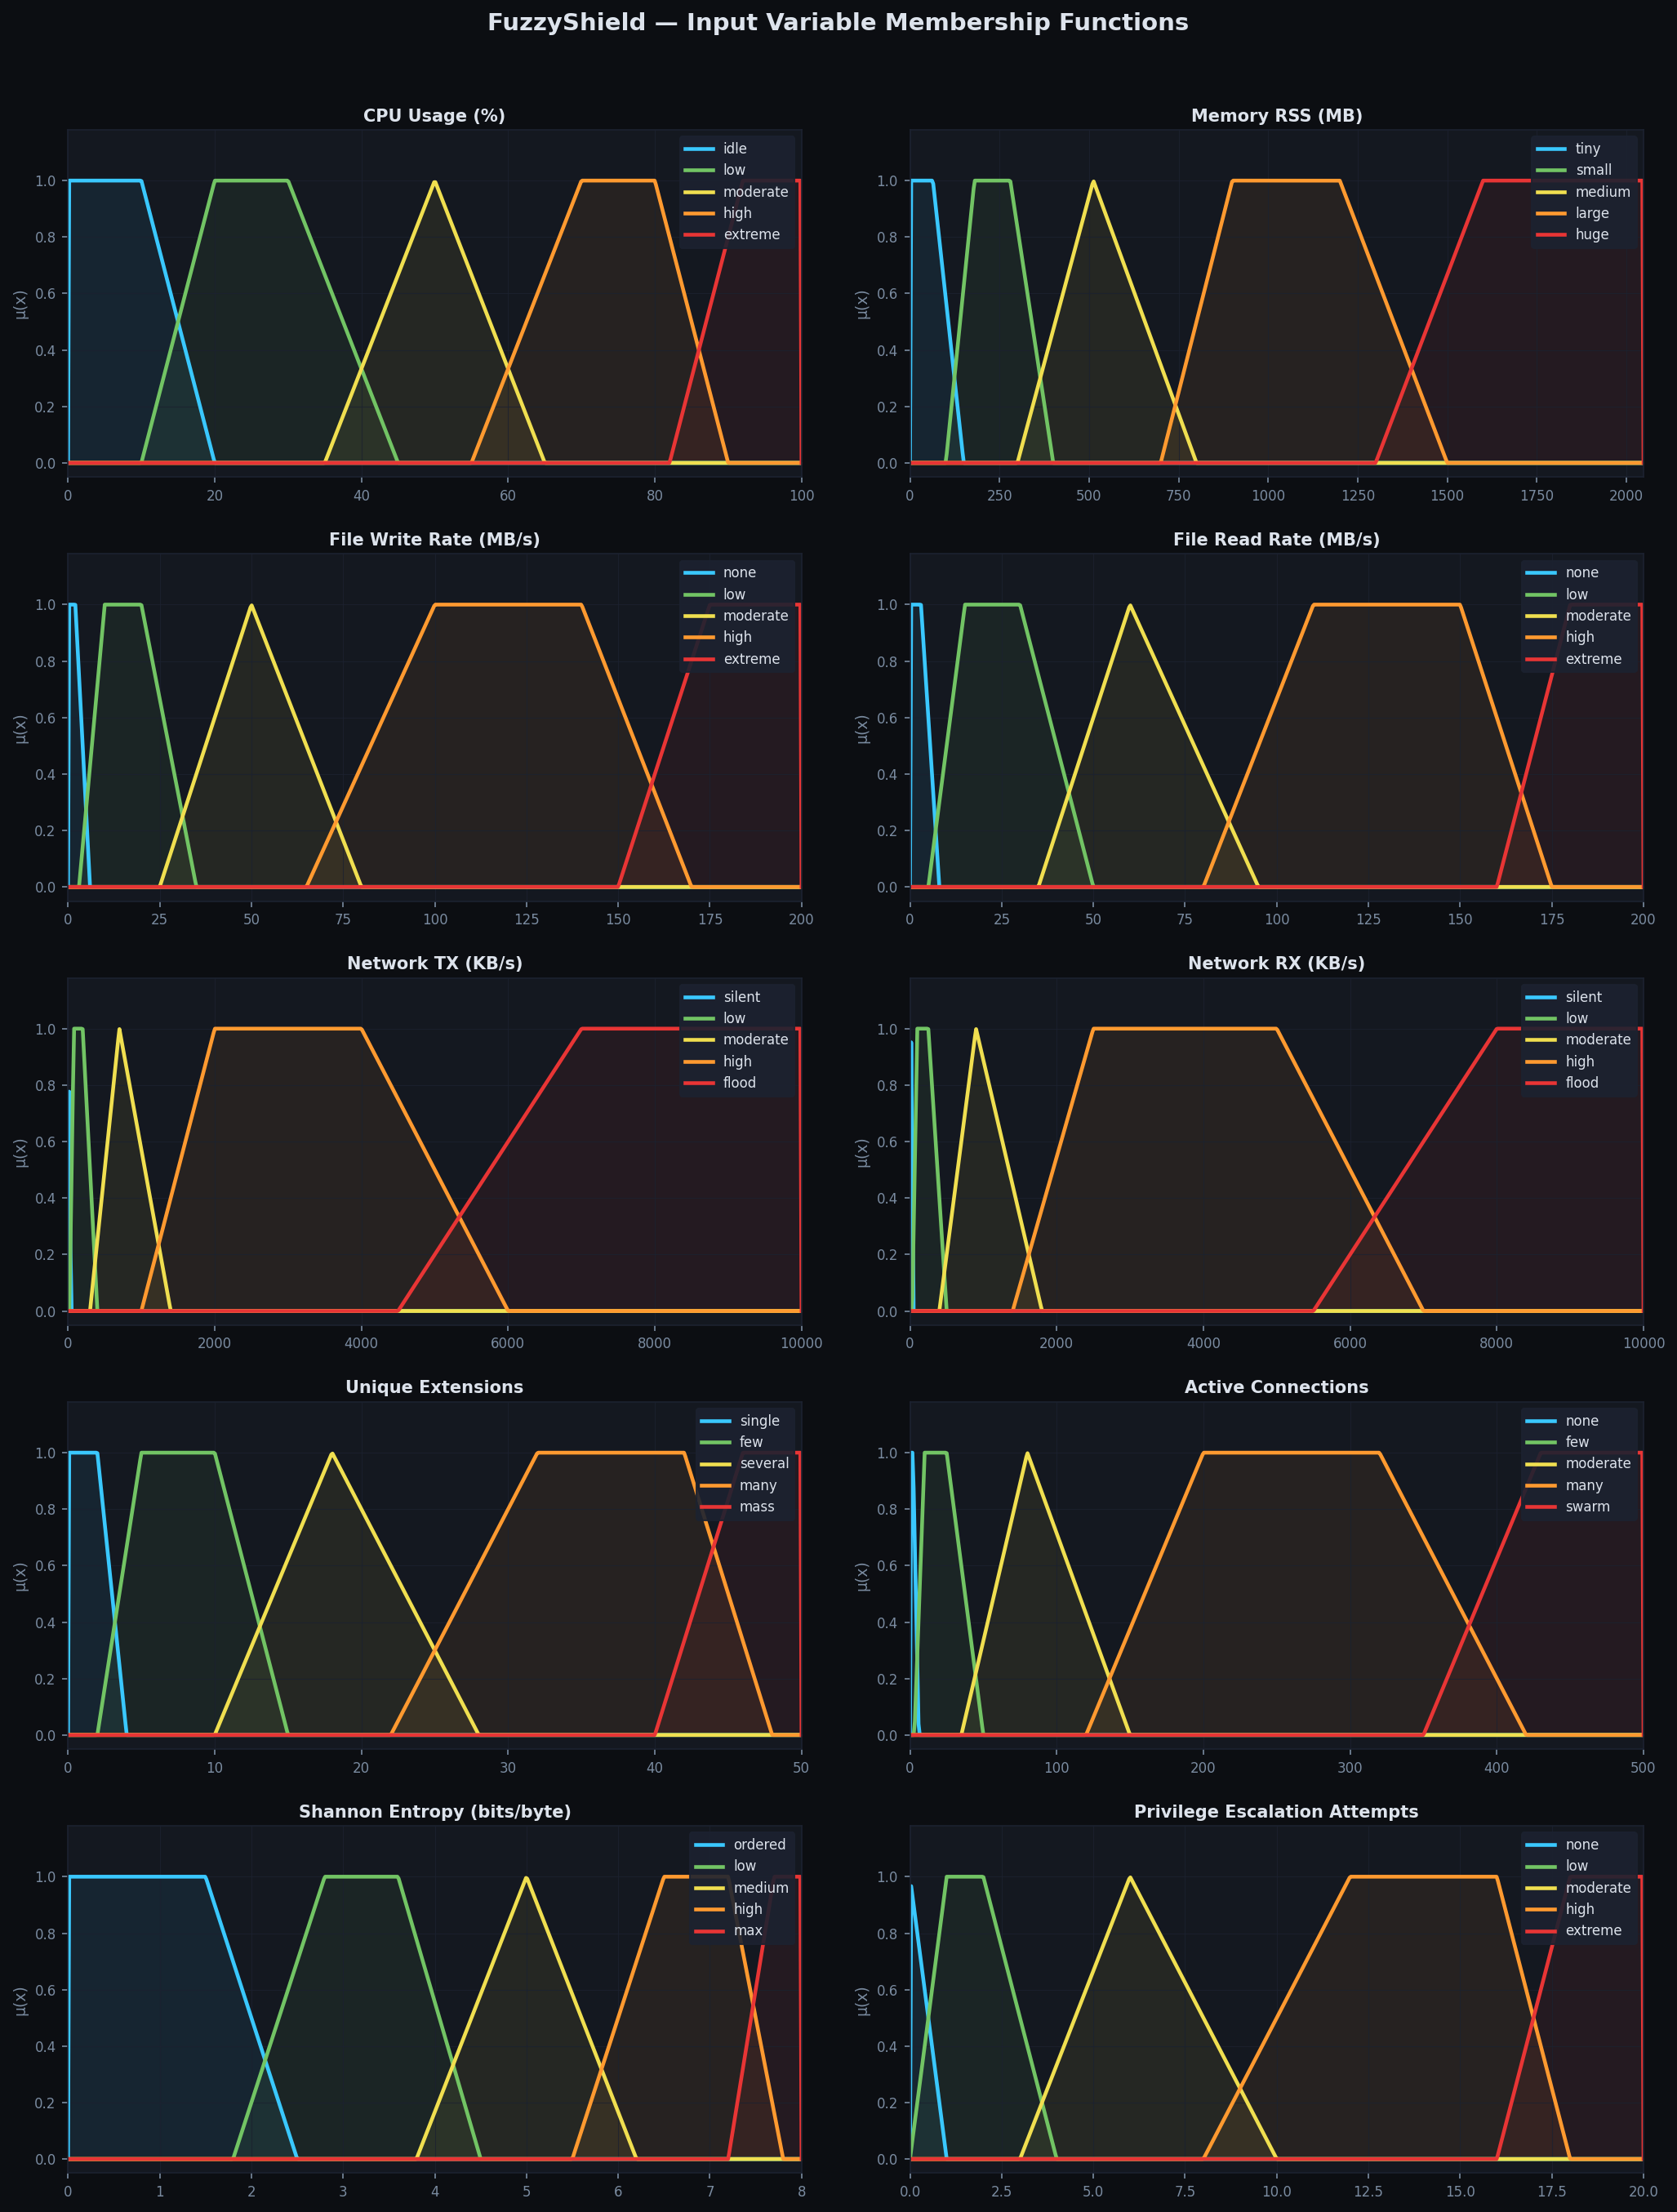
\includegraphics[width=\textwidth,
                       trim=0 780 0 0, clip]{figures/fig_mf_all_inputs.png}
    \end{column}
    \begin{column}{0.36\textwidth}
      \footnotesize
      \begin{itemize}\setlength{\itemsep}{5pt}
        \item \textbf{Trapezoidal} (\texttt{trapmf}) and \textbf{triangular}
              (\texttt{trimf}) MFs — overlapping boundaries for smooth transitions
        \item \texttt{cpu[extreme]}: starts at 82\% — real miners saturate \emph{all} cores
        \item \texttt{ent[max]}: $\geq7.2$\,bits/B — indistinguishable from AES output
        \item \texttt{conn[few]}: 3--50 conns — pool ($\approx$8) vs trojan swarms (300+)
      \end{itemize}
      \vspace{0.5em}
      \scriptsize\textit{Showing cpu, mem, fwrite, file\_read.\\All 10 MFs in report Fig.\ 2.}
    \end{column}
  \end{columns}
\end{frame}

\begin{frame}{Shannon Entropy — Key to Ransomware Detection}
  \begin{columns}[T]
    \begin{column}{0.50\textwidth}
      \begin{block}{Definition}
        \[
          H = -\sum_{b=0}^{255} p_b \log_2 p_b \quad \text{[bits/byte]}
        \]
      \end{block}
      \vspace{0.4em}
      \small
      \setlength{\tabcolsep}{5pt}
      \renewcommand{\arraystretch}{1.2}
      \begin{tabular}{@{} l c @{}}
        \toprule
        \textbf{Data type} & $H$ (bits/byte) \\
        \midrule
        Plain text (.txt)      & $\approx 4.5$ \\
        Executable (.exe)      & $\approx 6.0$ \\
        ZIP / compressed       & $\approx 7.5$ \\
        \R{AES ciphertext}     & $\approx \mathbf{7.9}$ \\
        \bottomrule
      \end{tabular}
    \end{column}
    \begin{column}{0.46\textwidth}
      \begin{exampleblock}{Measurement method}
        \small Reads \textbf{last 4\,KB} of open writable files,\\
        computes $H$ on byte value frequencies.
      \end{exampleblock}
      \vspace{0.35em}
      \begin{alertblock}{\texttt{ent[max]}: $H \geq 7.2$}
        \small
        Computationally indistinguishable from\\
        random data at this level.\\[0.25em]
        High \texttt{fwrite} + \texttt{ent[max]}\\
        $\Rightarrow$ \R{Ransomware CRITICAL}\\[0.25em]
        \textit{\C{Miner} contrast: pool uses\\
        \texttt{ent[low]} ($H<4.5$) — structured.}
      \end{alertblock}
    \end{column}
  \end{columns}
\end{frame}

\begin{frame}{Output Variables \& Verdict Generation}
  \begin{columns}[T]
    \begin{column}{0.46\textwidth}
      \begin{block}{3 Output Channels ($\in[0,1]$)}
        \footnotesize
        \setlength{\tabcolsep}{4pt}
        \renewcommand{\arraystretch}{1.15}
        \begin{tabular}{@{} l l @{}}
          \toprule
          \textbf{Term} & \textbf{Score range} \\
          \midrule
          none     & $< 15\%$ \\
          trace    & $5\%$–$35\%$ \\
          low      & $25\%$–$55\%$ \\
          medium   & $45\%$–$75\%$ \\
          high     & $65\%$–$92\%$ \\
          critical & $> 85\%$ \\
          \bottomrule
        \end{tabular}\\[0.4em]
        \footnotesize Centroid: $\;y^* = \tfrac{\int y\,\mu_{\text{agg}}\,dy}{\int \mu_{\text{agg}}\,dy}$
      \end{block}
    \end{column}
    \begin{column}{0.50\textwidth}
      \begin{alertblock}{Compound Verdict Algorithm}
        \footnotesize
        \begin{enumerate}\setlength{\itemsep}{1pt}
          \item $\max(R,T,C) < 0.10 \Rightarrow$ \G{BENIGN}
          \item $\max < 0.40 \Rightarrow$ \textcolor{orange}{SUSPICIOUS}
          \item Collect threats: score $\geq \max{-}0.05$\\
                AND score $\geq 0.35$\\
                $\Rightarrow$ join as \R{R}\,\texttt{+}\,\T{T}
          \item $\max \geq 0.70 \Rightarrow$ HIGH CONFIDENCE
        \end{enumerate}
      \end{alertblock}
      \vspace{0.3em}
      \begin{exampleblock}{Compound Example}
        \footnotesize
        R\,=\,50.6\%,\; T\,=\,51.0\%\\
        Both $\geq 35\%$, within $\Delta\!=\!5\%$\\
        $\Rightarrow$ \R{RANSOMWARE}\,\texttt{+}\,\T{TROJAN}
      \end{exampleblock}
    \end{column}
  \end{columns}
\end{frame}

\begin{frame}{Rule Base — 34 Mamdani Rules}
  \begin{columns}[T]
    \begin{column}{0.54\textwidth}
      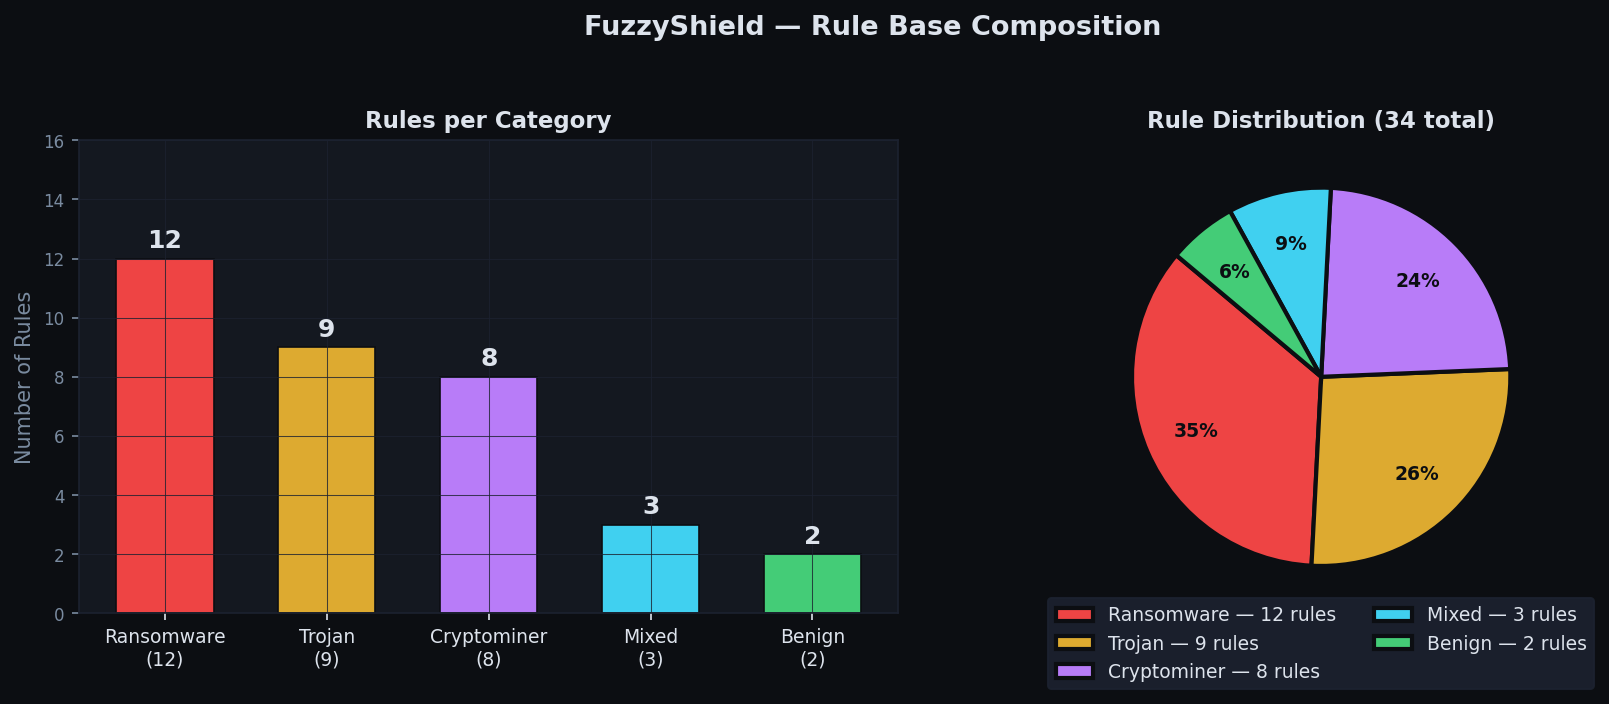
\includegraphics[width=\textwidth,
                       height=0.62\textheight,
                       keepaspectratio]{figures/fig_rule_dist.png}
    \end{column}
    \begin{column}{0.43\textwidth}
      \begin{block}{Rule structure}
        \footnotesize
        \textbf{IF} \textit{cond}\,AND\,\textit{cond}\ldots\\
        \textbf{THEN} \textit{output = term}\\[0.2em]
        Firing strength (min T-norm):\\
        $\alpha_k = \min_i \mu_{A_{ik}}(x_i)$
      \end{block}
      \vspace{0.35em}
      \begin{itemize}\footnotesize\setlength{\itemsep}{4pt}
        \item \R{12} Ransomware — fwrite, ext, ent
        \item \T{9}\phantom{0} Trojan — nettx, conn, priv
        \item \C{8}\phantom{0} Cryptominer — cpu, mem
        \item \M{3}\phantom{0} Mixed / ambiguous
        \item \G{2}\phantom{0} Benign suppression
      \end{itemize}
    \end{column}
  \end{columns}
\end{frame}

\begin{frame}{Key Rules — Ransomware}
  \begin{columns}[T]
    \begin{column}{0.54\textwidth}
      \footnotesize
      \setlength{\tabcolsep}{4pt}
      \renewcommand{\arraystretch}{1.25}
      \begin{tabular}{@{} c p{4.5cm} l @{}}
        \toprule
        \# & Antecedent & Output \\
        \midrule
        R1  & fwrite=\textit{extreme} \& ext=\textit{many} \& ent=\textit{max}
            & R=\textbf{critical} \\
        R2  & fwrite=\textit{high} \& ext=\textit{many} \& ent=\textit{high}
            & R=\textbf{high} \\
        R6  & fwrite=\textit{high} \& ent=\textit{max} \& priv=\textit{mod}
            & R=\textbf{high} \\
        R25 & fwrite=\textit{high} \& ext=\textit{several} \& ent=\textit{max}
            & R=\textbf{high} \\
        R27 & fwrite=\textit{high} \& ent=\textit{max} \& conn=\textit{none}
            & R=medium \\
        R28 & fwrite=\textit{extreme} \& fread=\textit{low} \& ent=\textit{max}
            & R=\textbf{critical} \\
        \bottomrule
      \end{tabular}
    \end{column}
    \begin{column}{0.42\textwidth}
      \begin{alertblock}{\small Design decisions}
        \footnotesize
        \textbf{R1 — strongest signal:}\\
        All three dominants active at once\\
        (write extreme + mass extensions\\
        + max entropy) = encrypt-in-place
        \vspace{0.3em}\\
        \textbf{R27 — offline case:}\\
        No C2 connection during encryption\\
        $\Rightarrow$ medium score, not critical
        \vspace{0.3em}\\
        \textbf{R28 — overwrite pattern:}\\
        Read little, write extreme + max ent\\
        = overwrite without reading first
      \end{alertblock}
    \end{column}
  \end{columns}
\end{frame}

\begin{frame}{Key Rules — Trojan \& Cryptominer}
  \begin{columns}[T]
    \begin{column}{0.48\textwidth}
      \begin{block}{Trojan rules}
        \scriptsize
        \setlength{\tabcolsep}{3pt}
        \renewcommand{\arraystretch}{1.1}
        \begin{tabular}{@{} c p{3.8cm} l @{}}
          \toprule
          \# & Antecedent & Out \\
          \midrule
          R8  & nettx=\textit{high} \& conn=\textit{many}
              \& priv=\textit{high}       & \textbf{crit.} \\
          R9  & nettx=\textit{flood} \& conn=\textit{swarm}
                                          & \textbf{crit.} \\
          R11 & cpu=\textit{low} \& conn=\textit{many}
              \& priv=\textit{high}       & high \\
          R14 & nettx=\textit{flood} \& priv=\textit{extreme}
                                          & \textbf{crit.} \\
          R30 & fread=\textit{low} \& nettx=\textit{high}
              \& conn=\textit{many}       & high \\
          \bottomrule
        \end{tabular}
      \end{block}
    \end{column}
    \begin{column}{0.48\textwidth}
      \setbeamercolor{block title}{bg=accent-c!80!black, fg=white}
      \setbeamercolor{block body}{bg=accent-c!10}
      \begin{block}{Cryptominer rules}
        \scriptsize
        \setlength{\tabcolsep}{3pt}
        \renewcommand{\arraystretch}{1.1}
        \begin{tabular}{@{} c p{4.0cm} l @{}}
          \toprule
          \# & Antecedent & Out \\
          \midrule
          R16 & cpu=\textit{extreme} \& fwrite=\textit{none}
              \& nettx=\textit{mod}       & \textbf{crit.} \\
          R17 & cpu=\textit{extreme} \& mem=\textit{large}
              \& nettx=\textit{mod}       & \textbf{crit.} \\
          R19 & cpu=\textit{extreme} \& fwrite=\textit{none}
              \& conn=\textit{few} \& ent=\textit{low} & high \\
          R22 & cpu=\textit{extreme} \& fwrite=\textit{none}
              \& conn=\textit{few}        & high \\
          R24 & cpu=\textit{extreme} \& fwrite=\textit{none}
              \& ent=\textit{ordered}     & \textbf{crit.} \\
          \bottomrule
        \end{tabular}
      \end{block}
      \vspace{0.1em}
      \scriptsize\textit{\texttt{conn[few]} prevents false positives\\
      from CPU-intensive non-miners.}
    \end{column}
  \end{columns}
\end{frame}

% ════════════════════════════════════════════════════════════════════════════
\section{Asymmetric EWMA}

\begin{frame}{Asymmetric EWMA — Temporal Feedback}
  \begin{columns}[T]
    \begin{column}{0.50\textwidth}
      \begin{block}{Update Rule (per check)}
        \[
          \hat{s}_t = \alpha\,\hat{s}_{t-1} + (1{-}\alpha)\,s_t
        \]
        \[
          \alpha = \begin{cases}
            \alpha_{\uparrow} = 0.15 & s_t \geq \hat{s}_{t-1}\\[3pt]
            \alpha_{\downarrow} = 0.85 & s_t < \hat{s}_{t-1}
          \end{cases}
        \]
      \end{block}
      \vspace{0.2em}
      \begin{itemize}\footnotesize\setlength{\itemsep}{3pt}
        \item \textbf{Rising} ($\alpha$=0.15): new value gets \textbf{85\%} weight\\
              $\Rightarrow$ threat alarm raised \textbf{in one window}
        \item \textbf{Falling} ($\alpha$=0.85): old score keeps \textbf{85\%}\\
              $\Rightarrow$ idle pause cannot reset alarm
        \item Defeats \alert{burst-pause evasion}:\\
              malware cannot hide by going briefly idle
        \item Verdict always on $\hat{s}_t$, not raw $s_t$
      \end{itemize}
    \end{column}
    \begin{column}{0.46\textwidth}
      \centering
      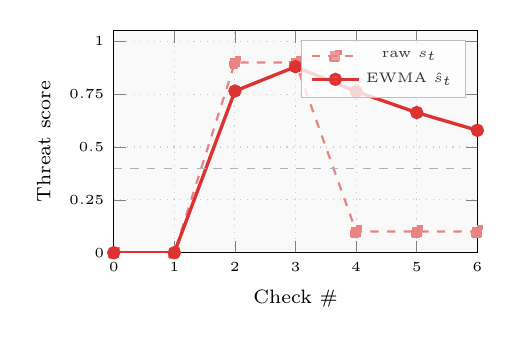
\begin{tikzpicture}[font=\scriptsize]
        \begin{axis}[
          width=6.2cm, height=4.4cm,
          xlabel={Check \#},
          ylabel={Threat score},
          ymin=0, ymax=1.05,
          xmin=0, xmax=6,
          xtick={0,1,2,3,4,5,6},
          ytick={0,0.25,0.5,0.75,1.0},
          yticklabel style={/pgf/number format/fixed,
                            /pgf/number format/precision=2},
          tick label style={font=\tiny},
          legend style={font=\tiny, at={(0.97,0.96)},
                        anchor=north east, fill=white, fill opacity=0.8,
                        draw=gray!50},
          grid=major, grid style={dotted, gray!40},
          axis background/.style={fill=gray!5},
        ]
          % Raw score: burst at checks 2–3, then idle
          \addplot[accent-r!60, dashed, thick,
                   mark=square*, mark size=1.8pt]
            coordinates {(0,0)(1,0)(2,0.9)(3,0.9)(4,0.1)(5,0.1)(6,0.1)};
          % EWMA smoothed
          % c0=0, c1=0, c2=0.765 (rise), c3=0.880 (rise),
          % c4=0.763 (fall), c5=0.663 (fall), c6=0.579 (fall)
          \addplot[accent-r, very thick,
                   mark=*, mark size=1.8pt]
            coordinates {(0,0)(1,0)(2,0.765)(3,0.880)
                          (4,0.763)(5,0.663)(6,0.579)};
          % Threshold line
          \addplot[gray!60, dashed, thin, domain=0:6] {0.4};
          \legend{raw $s_t$, EWMA $\hat{s}_t$}
        \end{axis}
      \end{tikzpicture}
      \vspace{0.1em}
      \scriptsize
      \begin{itemize}
        \item Checks 2--3: burst $\to$ score rises fast
        \item Check 4: process idles $\to$ score stays above 40\%
        \item \textit{Without EWMA: check 4 would drop to 10\%}
      \end{itemize}
    \end{column}
  \end{columns}
\end{frame}

% ════════════════════════════════════════════════════════════════════════════
\section{Implementation}

\begin{frame}{Dual Implementation: Python \& MATLAB}
  \begin{columns}[T]
    \begin{column}{0.48\textwidth}
      \begin{block}{Python — \texttt{scikit-fuzzy}}
        \begin{itemize}\footnotesize\setlength{\itemsep}{2pt}
          \item \texttt{skfuzzy.control} Mamdani API
          \item \texttt{psutil} live PID monitoring
          \item \texttt{/proc/pid/io wchar} write rate
          \item Timestamped: \texttt{scenarios/},
                \texttt{pid\_sessions/}, \texttt{analysis/}
          \item Behavioral simulator: \texttt{sim/malware\_sim.py}
        \end{itemize}
      \end{block}
    \end{column}
    \begin{column}{0.48\textwidth}
      \begin{block}{MATLAB — Fuzzy Logic Toolbox}
        \begin{itemize}\footnotesize\setlength{\itemsep}{2pt}
          \item \texttt{mamfis} API, \texttt{addRule}
          \item \textbf{Exact mirror} of 34 Python rules
          \item Exports \texttt{FuzzyShield.fis} (Fuzzy Logic Designer)
          \item 3D surface plots via \texttt{evalfis}
          \item Identical MF parameters $\Rightarrow$ same outputs
        \end{itemize}
      \end{block}
    \end{column}
  \end{columns}
  \vspace{0.1em}
  \begin{block}{Behavioral Simulator — \texttt{sim/malware\_sim.py}}
    \scriptsize
    \setlength{\tabcolsep}{5pt}
    \renewcommand{\arraystretch}{1.05}
    \begin{tabular}{@{} l p{9.5cm} @{}}
      \R{Ransomware}  & 8 workers $\times$ 500\,KB \texttt{os.urandom()}, 20 ext., held 40\,ms \\
      \T{Trojan}      & 250 loopback TCP conns, echo server, $\approx$25\,MB/s TX/RX \\
      \C{Cryptominer} & $N_\text{cores}$ SHA-256 threads + 8 pool connections ($\approx$640\,KB/s)\\
      \G{Benign}      & idle sleep loop, minimal resource use \\
    \end{tabular}
  \end{block}
\end{frame}

% ════════════════════════════════════════════════════════════════════════════
\section{Results}

\begin{frame}{Preset Scenario Results}
  \begin{columns}[T]
    \begin{column}{0.42\textwidth}
      \footnotesize
      \setlength{\tabcolsep}{4pt}
      \renewcommand{\arraystretch}{1.2}
      \begin{tabular}{@{} l c c c @{}}
        \toprule
        \textbf{Scenario} & \textbf{R\%} & \textbf{T\%} & \textbf{C\%} \\
        \midrule
        \R{Ransomware}  & \R{\textbf{83.5}} & 14.1 &  6.6 \\
        \T{Trojan}      & 15.7 & \T{\textbf{76.3}} & 15.7 \\
        \C{Cryptominer} &  5.4 &  5.4 & \C{\textbf{83.7}} \\
        \G{Benign}      &  6.6 &  6.6 &  6.6 \\
        \M{Mixed}       & \R{\textbf{50.6}} & \T{\textbf{51.0}} & 9.0 \\
        \bottomrule
      \end{tabular}
      \vspace{0.3em}
      \begin{itemize}\footnotesize
        \item All 4 single threats $\geq$70\%:\\
              \textbf{HIGH CONFIDENCE}
        \item Benign $<$10\%: \G{SAFE}
        \item Mixed: \R{R}\,\textbf{+}\,\T{T} compound
      \end{itemize}
    \end{column}
    \begin{column}{0.55\textwidth}
      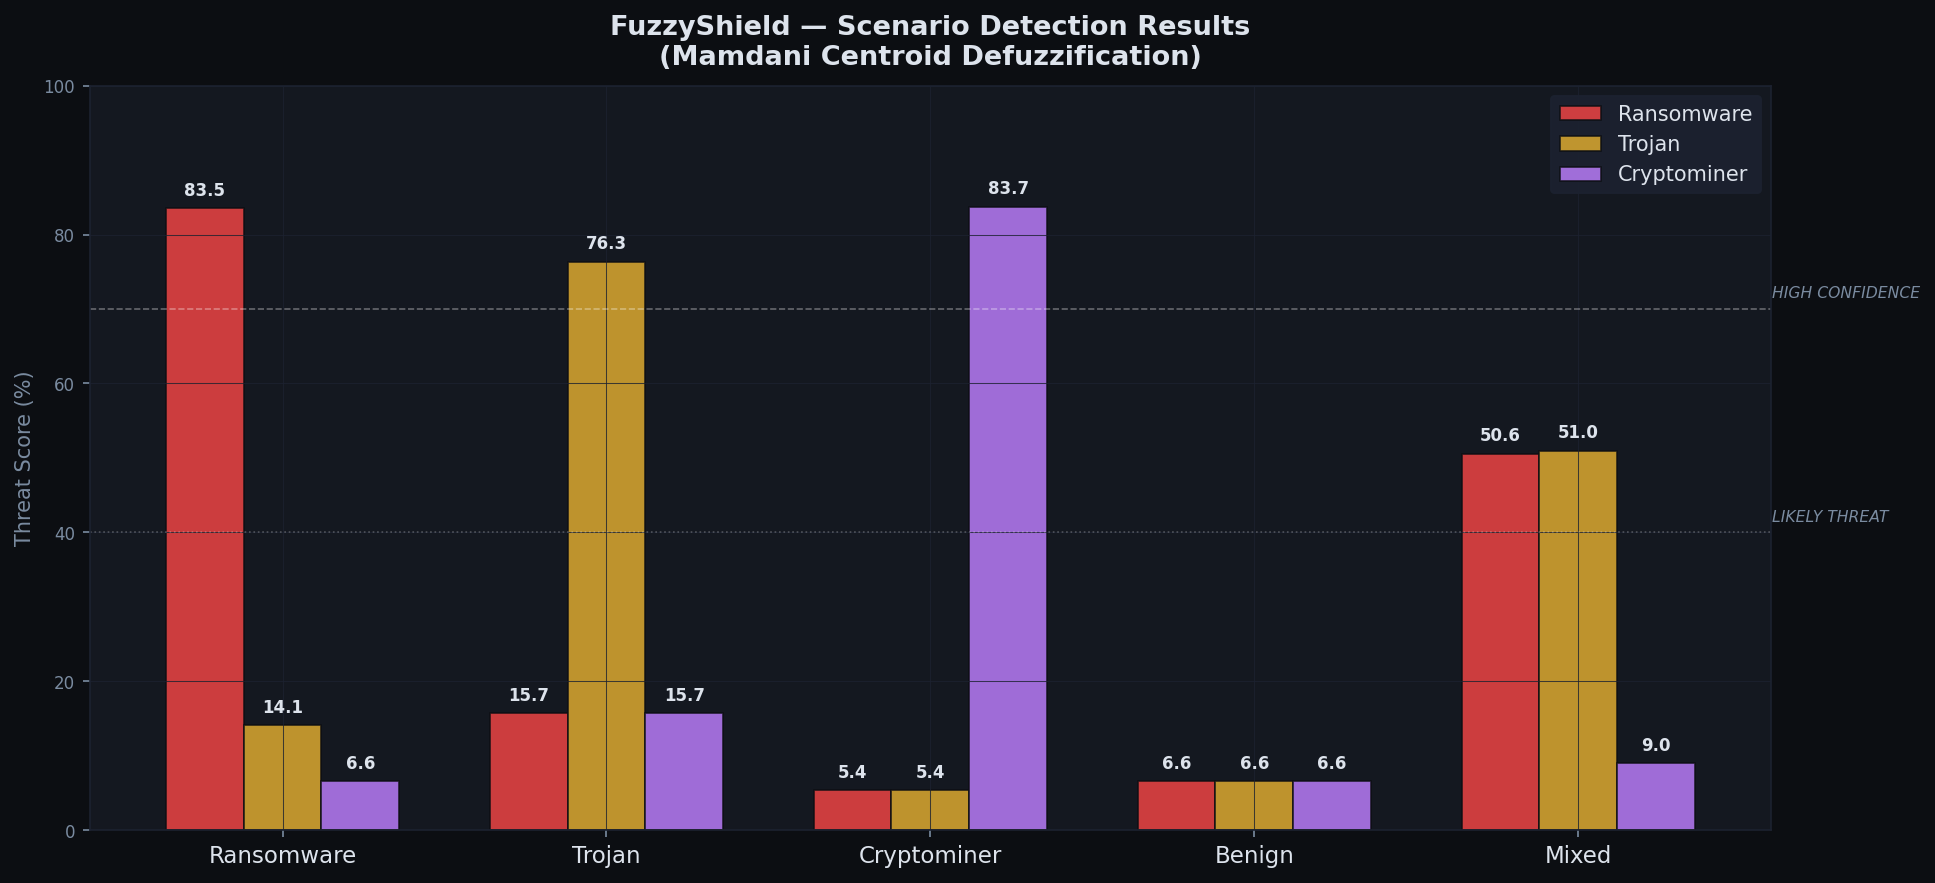
\includegraphics[width=\textwidth,
                       height=0.70\textheight,
                       keepaspectratio]{figures/fig_results.png}
    \end{column}
  \end{columns}
\end{frame}

\begin{frame}{Why Each Scenario Fires}
  \begin{columns}[T]
    \begin{column}{0.48\textwidth}
      \begin{alertblock}{\small Ransomware — 83.5\%}
        \footnotesize
        \begin{tabular}{@{}ll@{}}
          fwrite & 160 MB/s (\textit{extreme}) \\
          ext    & 45 (\textit{mass}) \\
          ent    & 7.8 (\textit{max}) \\
        \end{tabular}\\
        Rules fired: R1, R2, R5, R25, R28
      \end{alertblock}
      \vspace{0.1em}
      \begin{block}{\small Trojan — 76.3\%}
        \footnotesize
        \begin{tabular}{@{}ll@{}}
          nettx & 4200 KB/s (\textit{high}) \\
          conn  & 320 (\textit{many}) \\
          priv  & 14 (\textit{high}) \\
        \end{tabular}\\
        Rules fired: R8, R9, R10, R12
      \end{block}
    \end{column}
    \begin{column}{0.48\textwidth}
      \setbeamercolor{block title}{bg=accent-c!80!black, fg=white}
      \setbeamercolor{block body}{bg=accent-c!10}
      \begin{block}{\small Cryptominer — 83.7\%}
        \footnotesize
        \begin{tabular}{@{}ll@{}}
          cpu    & 96\% (\textit{extreme}) \\
          mem    & 1400 MB (\textit{huge}) \\
          fwrite & 2 MB/s (\textit{none}) \\
          conn   & 20 (\textit{few}) \\
        \end{tabular}\\
        Rules fired: R16, R17, R20, R22
      \end{block}
      \vspace{0.1em}
      \begin{exampleblock}{\small Benign — 6.6\%}
        \footnotesize
        \begin{tabular}{@{}ll@{}}
          cpu   & 12\% (\textit{idle}) \\
          fwrite & 4 MB/s (\textit{none}) \\
          conn  & 4 (\textit{none}) \\
        \end{tabular}\\
        Rules B1, B2 $\to$ all outputs suppressed
      \end{exampleblock}
    \end{column}
  \end{columns}
\end{frame}

\begin{frame}{Compound Threat Detection}
  \begin{columns}[T]
    \begin{column}{0.53\textwidth}
      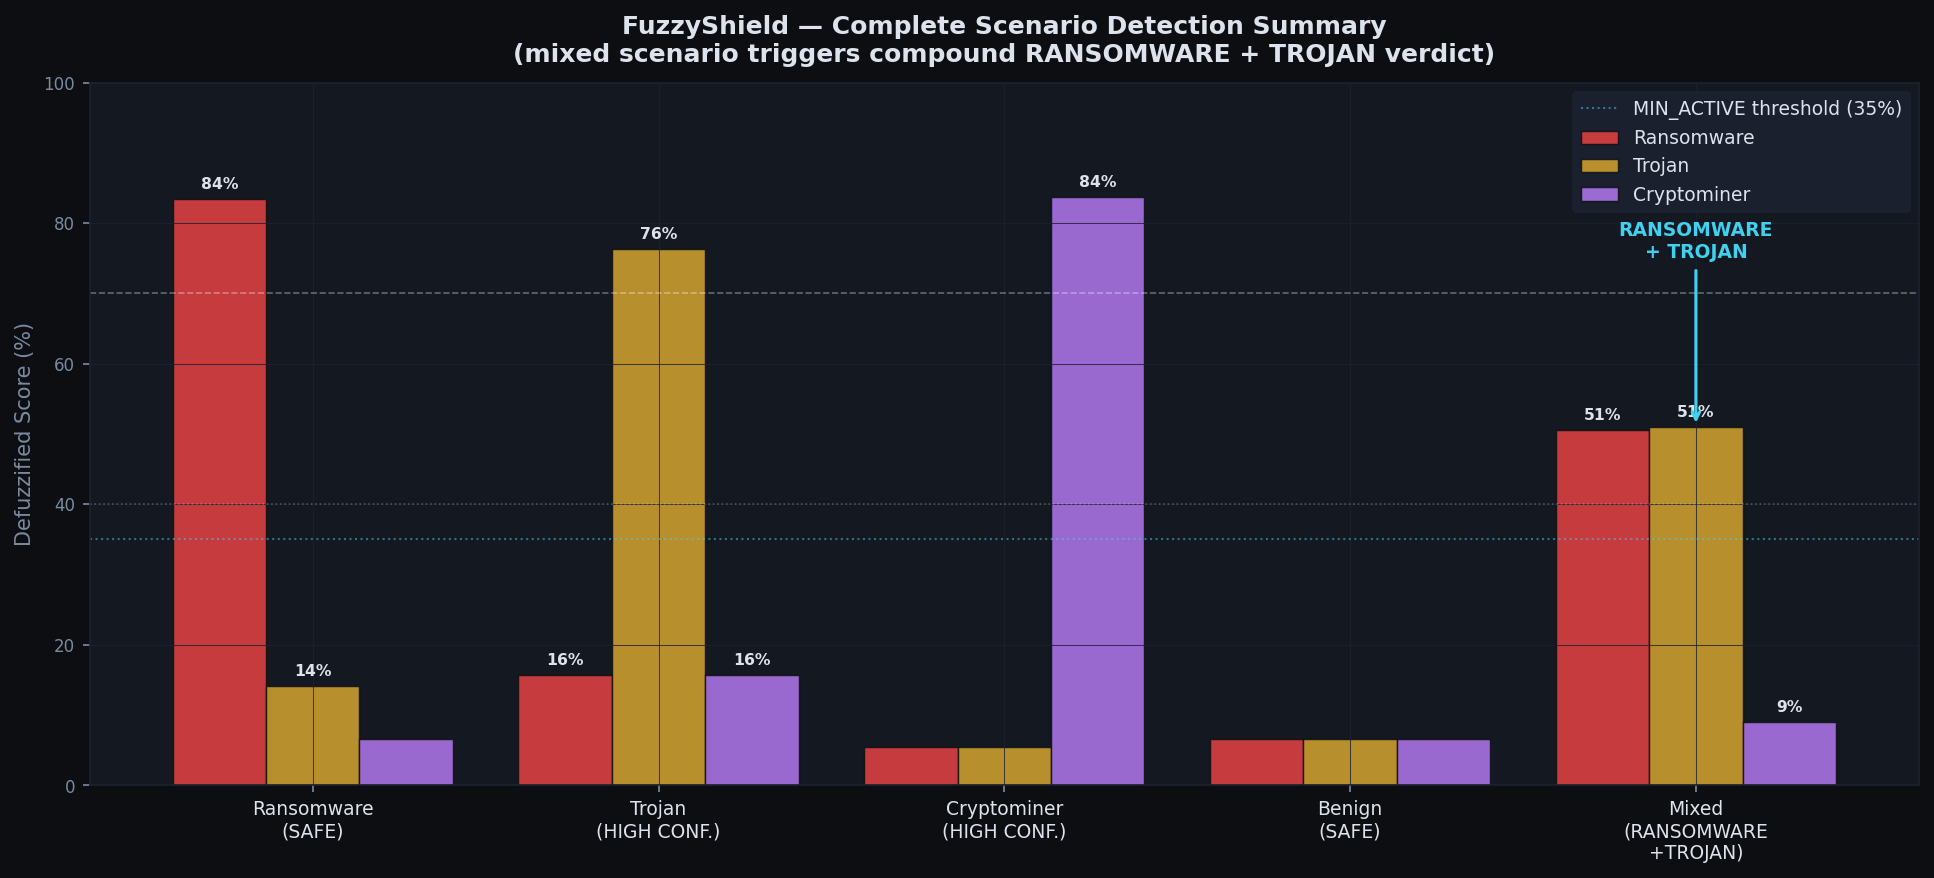
\includegraphics[width=\textwidth,
                       height=0.72\textheight,
                       keepaspectratio]{figures/fig_compound.png}
    \end{column}
    \begin{column}{0.43\textwidth}
      \begin{block}{\small Mixed Scenario Inputs}
        \footnotesize
        \begin{tabular}{@{}ll@{}}
          fwrite & 170 MB/s (\textit{extreme}) \\
          ent    & 7.8 (\textit{max}) \\
          ext    & 38 (\textit{many}) \\
          nettx  & 1800 KB/s (\textit{high}) \\
          conn   & 180 (\textit{many}) \\
          priv   & 10 (\textit{high}) \\
        \end{tabular}
      \end{block}
      \vspace{0.3em}
      \begin{alertblock}{\small Verdict}
        \small
        R\,=\,\R{\textbf{50.6\%}},\; T\,=\,\T{\textbf{51.0\%}}\\
        Both $\geq 35\%$, $\Delta < 5\%$\\[0.15em]
        $\Rightarrow$ \R{RANSOMWARE}\,\textbf{+}\,\T{TROJAN}\\
        \footnotesize\textit{LIKELY THREAT}\\[0.1em]
        \scriptsize Rule M3: priv\,+\,ent\,+\,conn fires both channels.
      \end{alertblock}
    \end{column}
  \end{columns}
\end{frame}

\begin{frame}{3D Rule Surfaces (MATLAB Surface Viewer)}
  \begin{center}
    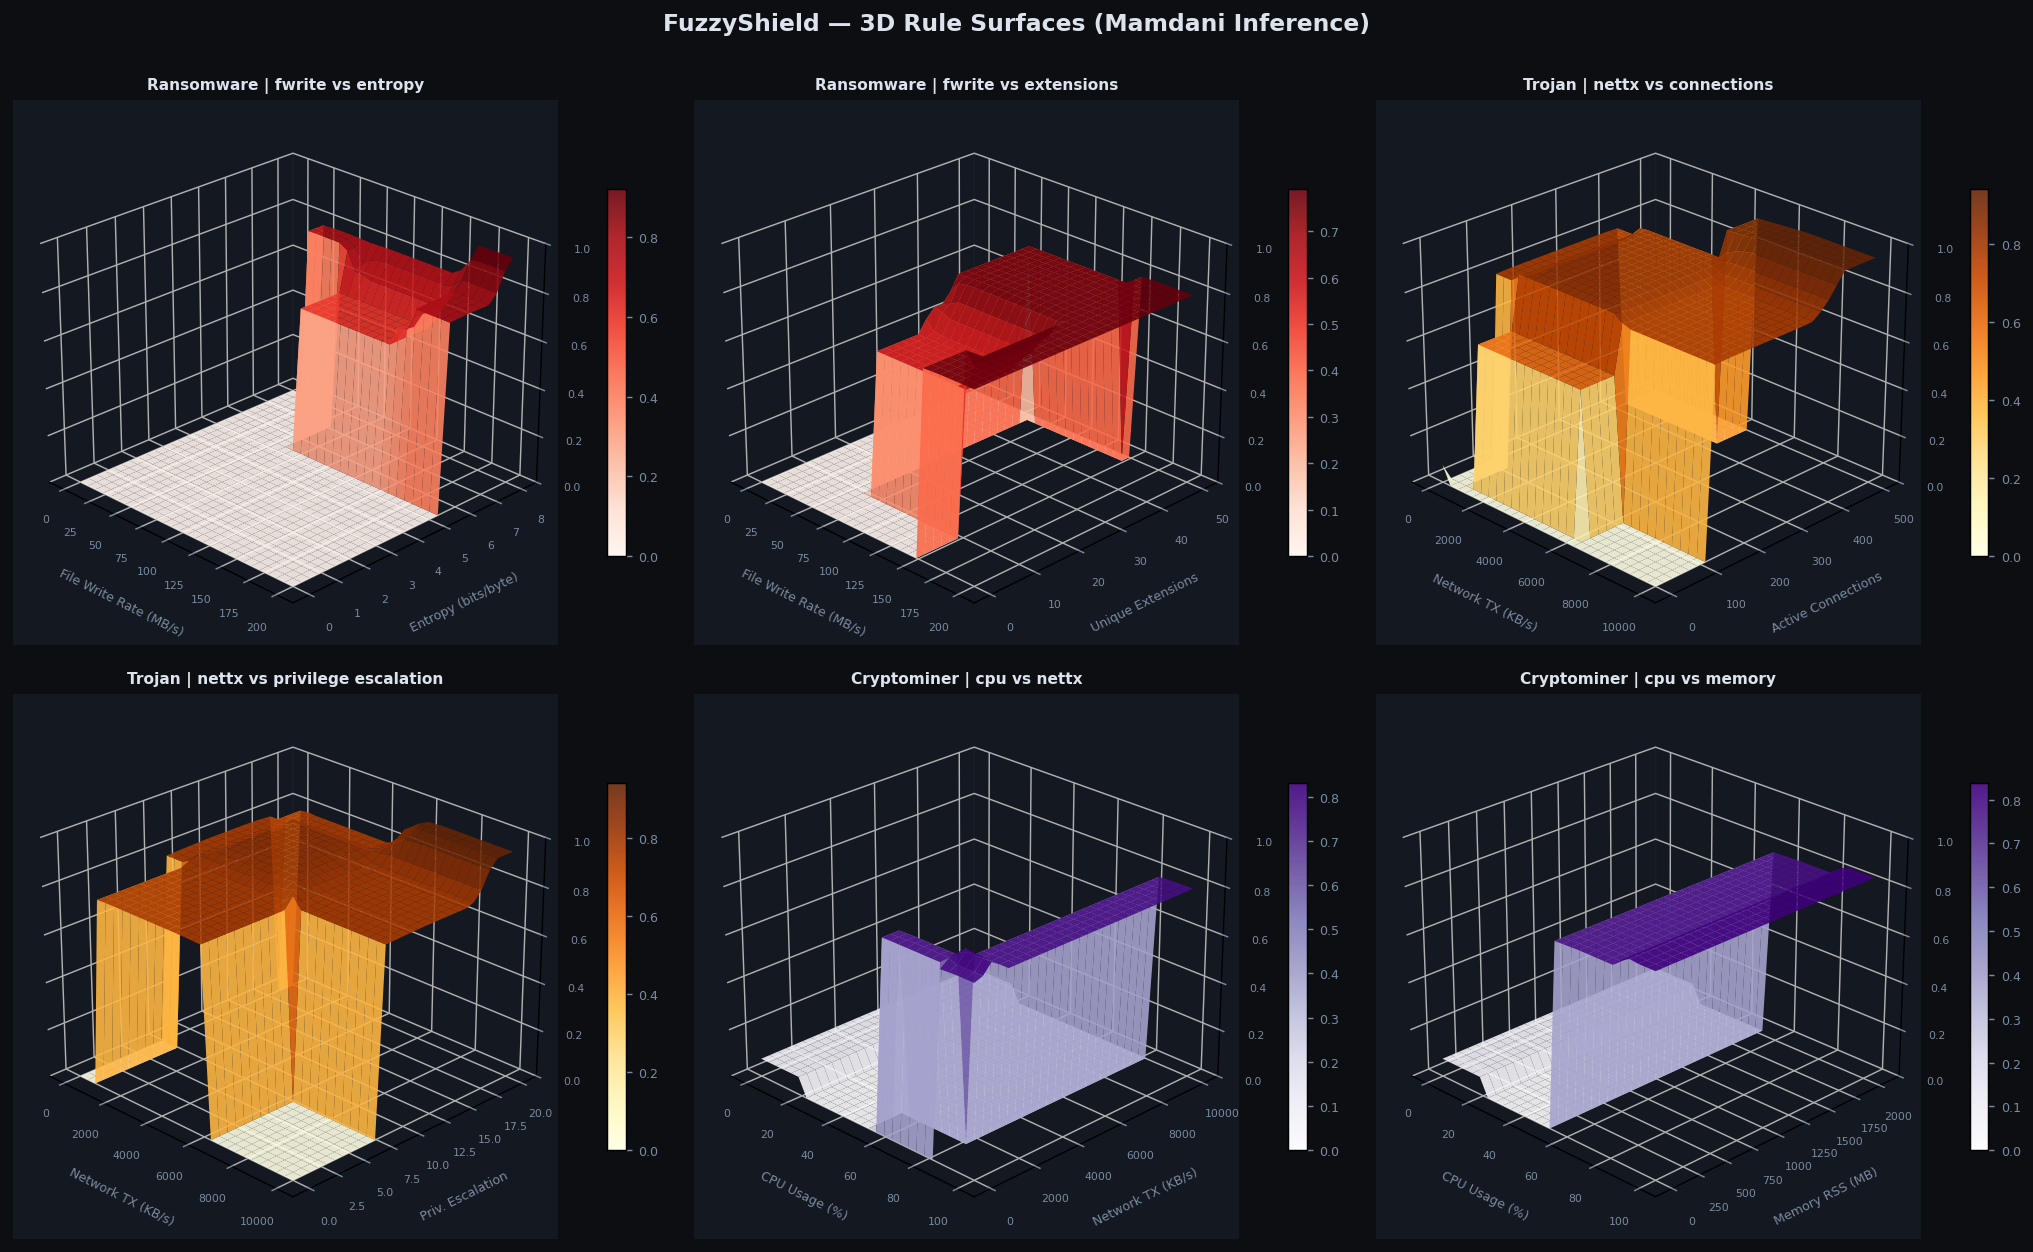
\includegraphics[width=0.97\textwidth,
                     height=0.68\textheight,
                     keepaspectratio]{figures/fig_surfaces.png}
  \end{center}
  \vspace{-0.3em}
  \begin{columns}
    \begin{column}{0.32\textwidth}
      \centering\footnotesize
      \R{Ransomware}:\\
      Sharp ridge — fwrite \& ent\\
      must \emph{both} exceed ``high''
    \end{column}
    \begin{column}{0.32\textwidth}
      \centering\footnotesize
      \T{Trojan}:\\
      Plateau at high nettx\\
      \& many connections
    \end{column}
    \begin{column}{0.32\textwidth}
      \centering\footnotesize
      \C{Cryptominer}:\\
      Narrow ridge: cpu=extreme\\
      + nettx=moderate (pool)
    \end{column}
  \end{columns}
\end{frame}

% ════════════════════════════════════════════════════════════════════════════
\section{Conclusion}

\begin{frame}{Conclusion}
  \begin{columns}[T]
    \begin{column}{0.50\textwidth}
      \begin{block}{What was built}
        \begin{itemize}\footnotesize\setlength{\itemsep}{1pt}
          \item Mamdani FIS: \textbf{10 inputs, 3 outputs, 34 rules}
          \item Real-time \texttt{psutil}-based PID monitor
          \item Compound verdict (multi-threat)
          \item Asymmetric EWMA ($\alpha_{\uparrow}$=0.15, $\alpha_{\downarrow}$=0.85)
          \item Python + MATLAB dual implementations
        \end{itemize}
      \end{block}
      \vspace{0.1em}
      \begin{block}{Detection accuracy}
        \scriptsize
        \setlength{\tabcolsep}{3pt}
        \renewcommand{\arraystretch}{1.0}
        \begin{tabular}{@{} l c c @{}}
          \toprule
          Threat & Score & Verdict \\
          \midrule
          \R{Ransomware}  & 83.5\% & HIGH CONF. \\
          \T{Trojan}      & 76.3\% & HIGH CONF. \\
          \C{Cryptominer} & 83.7\% & HIGH CONF. \\
          \G{Benign}      &  6.6\% & SAFE \\
          \bottomrule
        \end{tabular}
      \end{block}
    \end{column}
    \begin{column}{0.46\textwidth}
      \begin{alertblock}{Limitations}
        \begin{itemize}\footnotesize\setlength{\itemsep}{1pt}
          \item Web servers can mimic miner CPU profile
          \item Single-window snapshot $\to$ FP risk
          \item Async write buffers may delay entropy
        \end{itemize}
      \end{alertblock}
      \vspace{0.1em}
      \begin{exampleblock}{Future Work}
        \begin{itemize}\footnotesize\setlength{\itemsep}{1pt}
          \item Adaptive MF tuning via RL
          \item Trend-based temporal features
          \item eBPF kernel integration
          \item Wider taxonomy: worms, rootkits
        \end{itemize}
      \end{exampleblock}
    \end{column}
  \end{columns}
\end{frame}

% ── THANK YOU ────────────────────────────────────────────────────────────────
\begin{frame}[plain]
  \begin{center}
    \vspace{1.2em}
    {\Huge \color{iyte-blue}\textbf{Thank You}}\\[0.6em]
    {\large Questions?}\\[1.6em]
    
\includegraphics[height=1.4cm]{figures/iyte_logo.png}\\[0.7em]
    {\small Ahmet Faruk Kesgin \quad \mbox{300201024}}\\
    {\small Department of Computer Engineering}\\
    {\small Izmir Institute of Technology}\\[0.5em]
    \rule{6cm}{0.4pt}\\[0.4em]
    {\small\color{iyte-blue}
      \url{https://github.com/Farukesgin/FuzzyShield}}\\[0.3em]
    {\footnotesize\color{iyte-blue}
      \textbf{FuzzyShield} — Real-Time Behavioral Malware Classification\\
      Using Fuzzy Logic \;|\; June 2026}
  \end{center}
\end{frame}

\end{document}
